\documentclass[conference]{IEEEtran}
\IEEEoverridecommandlockouts

\usepackage[T1]{fontenc}
\usepackage{cite}
\usepackage{amsmath,amssymb,amsfonts}
\usepackage{graphicx}
\usepackage{textcomp}
\usepackage{xcolor}
\usepackage{booktabs}
\usepackage{placeins}
\usepackage{flushend}

\def\BibTeX{{\rm B\kern-.05em{\sc i\kern-.025em b}\kern-.08em
    T\kern-.1667em\lower.7ex\hbox{E}\kern-.125emX}}
\begin{document}

\title{ClinCode Copilot: An Interactive Clinical Coding Assistant with Dual Interpretability}

\author{\IEEEauthorblockN{1\textsuperscript{st} Lu\'{i}s Carlos Afonso}
\IEEEauthorblockA{0009-0005-6728-3089}
\and
\IEEEauthorblockN{2\textsuperscript{nd} Vicente Barros}
\IEEEauthorblockA{0009-0007-4526-2249}
\and
\IEEEauthorblockN{3\textsuperscript{rd} Jo\~{a}o Rafael Almeida}
\IEEEauthorblockA{0000-0003-0729-2264}
\and
\IEEEauthorblockN{4\textsuperscript{th} Jos\'{e} Lu\'{i}s Oliveira}
\IEEEauthorblockA{0000-0002-6672-6176}
}

\maketitle

\begin{abstract}
The assignment of International Classification of Diseases (ICD) codes to clinical encounters is a labor-intensive process that is both error-prone and costly. While automated coding models have made substantial progress on benchmark datasets, they typically operate as batch-oriented black boxes that produce ranked code lists without supporting evidence. Clinical coders, however, require interactive tools that explain predictions in terms they can verify against the source document. We present ClinCode Copilot, a web-based clinical coding assistant that integrates a hybrid machine learning model with an interactive workspace designed for real-time ICD code review. The system combines an end-to-end label attention classifier with chunk-level K-nearest neighbor retrieval to provide dual interpretability: per-code attention highlighting identifies which sections of a discharge summary support each prediction, while similar patient retrieval surfaces training cases that received the same code. Built with a FastAPI backend serving a Bio\_ClinicalBERT encoder and FAISS index, and a Next.js frontend with resizable multi-panel layout, ClinCode Copilot enables clinical coders to review predictions, inspect evidence, and verify codes within a single interface. The underlying model achieves Micro-F1 of 0.482 on 1,275 ICD-9 codes from MIMIC-III.
\end{abstract}

\begin{IEEEkeywords}
clinical coding, ICD, clinical decision support, interpretable AI, attention visualization, case-based reasoning, web application
\end{IEEEkeywords}

\section{Introduction}

The assignment of International Classification of Diseases (ICD) codes to clinical encounters is fundamental to healthcare operations, supporting reimbursement, epidemiological surveillance, and quality measurement. In the United States alone, medical coders process millions of discharge summaries annually, selecting from over 14,000 ICD-9 categories or the even larger ICD-10 vocabulary. This process is labor-intensive, error-prone, and costly, with studies estimating error rates between 10\% and 30\% even among experienced coders~\cite{b_omalley2005, b_burns2012}.

Automated ICD coding has made substantial progress. Neural methods such as CAML~\cite{b_mullenbach2018}, LAAT~\cite{b_vu2020}, and PLM-ICD~\cite{b_plmicd} achieve strong performance on benchmark datasets by fine-tuning deep neural networks with per-label attention mechanisms. However, these systems function as batch-oriented classifiers that accept a document and return a ranked list of codes without interactive explanation. In clinical practice, a prediction without supporting evidence has limited value: coders must understand \emph{why} a code was suggested to verify its correctness and to satisfy audit requirements~\cite{b_topaz2013}.

The gap between research systems and clinical workflow is twofold. First, existing models lack the interactive capabilities that coders need---the ability to select a predicted code and immediately see the supporting evidence in the source document. Second, even systems that provide attention-based explanations typically offer token-level highlights that scatter across the document rather than identifying coherent clinical sections. Clinical coders think in terms of document sections (``the cardiac workup supports this diagnosis''), not individual tokens.

We present ClinCode Copilot, a web-based clinical coding assistant designed to bridge this gap. The system integrates a hybrid machine learning model---combining end-to-end label attention with chunk-level K-nearest neighbor (KNN) retrieval---into an interactive workspace that supports the clinical coding workflow. ClinCode Copilot provides two complementary forms of explanation for every predicted code: (a) chunk-level attention highlighting that identifies which sections of the discharge summary support the prediction, rendered as a heat-map overlay on the source text; and (b) similar patient retrieval that surfaces training cases receiving the same code, enabling case-based verification.

The system is built as a full-stack web application. A FastAPI backend serves a Bio\_ClinicalBERT encoder with a per-code chunk attention head and a FAISS index containing approximately 793K training chunk embeddings. A Next.js frontend provides a multi-panel resizable workspace where coders can enter discharge text, review predictions with confidence scores, inspect attention highlights, and examine similar patients---all within a single interface.

We make three contributions: (a) an interactive system that integrates a hybrid ICD coding model with a clinical coding workflow, providing real-time predictions with dual explanations; (b) a dual interpretability approach combining chunk-level attention visualization with case-based retrieval, offering complementary evidence modalities for code verification; and (c) a system architecture that enables real-time inference on clinical-length documents through efficient chunking, batched encoding, and approximate nearest-neighbor search.

\section{Related Work}

\subsection{Clinical NLP tools}

Several systems have been developed for clinical text processing. cTAKES~\cite{b_ctakes} provides a pipeline for named entity recognition and concept extraction from clinical narratives using rule-based and machine learning components. MedCAT~\cite{b_medcat} offers concept annotation and linking to medical ontologies with active learning capabilities. These tools focus on entity-level extraction rather than document-level code assignment and do not provide the interactive prediction-and-verification workflow that clinical coders require.

\subsection{Automated ICD coding}

The dominant paradigm for automated ICD coding uses per-label attention over neural document representations. CAML~\cite{b_mullenbach2018} introduced code-specific attention over CNN features, LAAT~\cite{b_vu2020} extended this with a bidirectional LSTM encoder, and PLM-ICD~\cite{b_plmicd} applied the pattern to pre-trained language models. MSMN~\cite{b_yuan2022} further improved performance by aligning code representations with UMLS synonyms. While these methods achieve strong benchmark performance, they function as offline classifiers without interactive explanation capabilities. Our system deploys such a model within an interactive tool that surfaces its internal attention weights as user-facing explanations.

\subsection{Explainable clinical AI}

Interpretability in clinical NLP has been pursued through attention visualization~\cite{b_mullenbach2018, b_vu2020}, feature attribution methods such as LIME~\cite{b_lime} and SHAP~\cite{b_shap}, and case-based reasoning~\cite{b_kolodner1992}. Attention weights, while debated as faithful explanations~\cite{b_jain2019, b_wiegreffe2019}, provide useful indicative signals for clinical review when operating at an appropriate granularity. Case-based reasoning---explaining a prediction by retrieving similar cases---has a long history in medical decision support~\cite{b_bichindaritz2006} and aligns with how clinical coders naturally verify codes against their experience. Our system combines both approaches, providing attention-based and retrieval-based explanations simultaneously.

\subsection{Clinical decision support systems}

Clinical decision support systems (CDSS) have evolved from rule-based expert systems to machine learning-driven tools integrated into electronic health records~\cite{b_sutton2020}. Effective CDSS design requires not only accurate predictions but also transparency, integration with clinical workflows, and appropriate levels of automation~\cite{b_sittig2020}. ClinCode Copilot follows these principles by positioning the ML model as a suggestion tool that supports rather than replaces the coder's judgment, with dual explanations that enable informed acceptance or rejection of each prediction.

\section{System Architecture}

\subsection{Overview}

ClinCode Copilot follows a client-server architecture with a clear separation between the ML inference backend and the interactive frontend (Fig.~\ref{fig:ui_overview}). A discharge summary enters the system through the frontend text input, is transmitted to the backend API, preprocessed and segmented into overlapping chunks, encoded by a BERT model, scored by both a label attention classifier and a KNN retrieval module, and returned to the frontend where predictions are displayed alongside interactive attention highlighting and similar patient information. The full pipeline executes synchronously, enabling real-time interaction.

\begin{figure*}[t]
\centerline{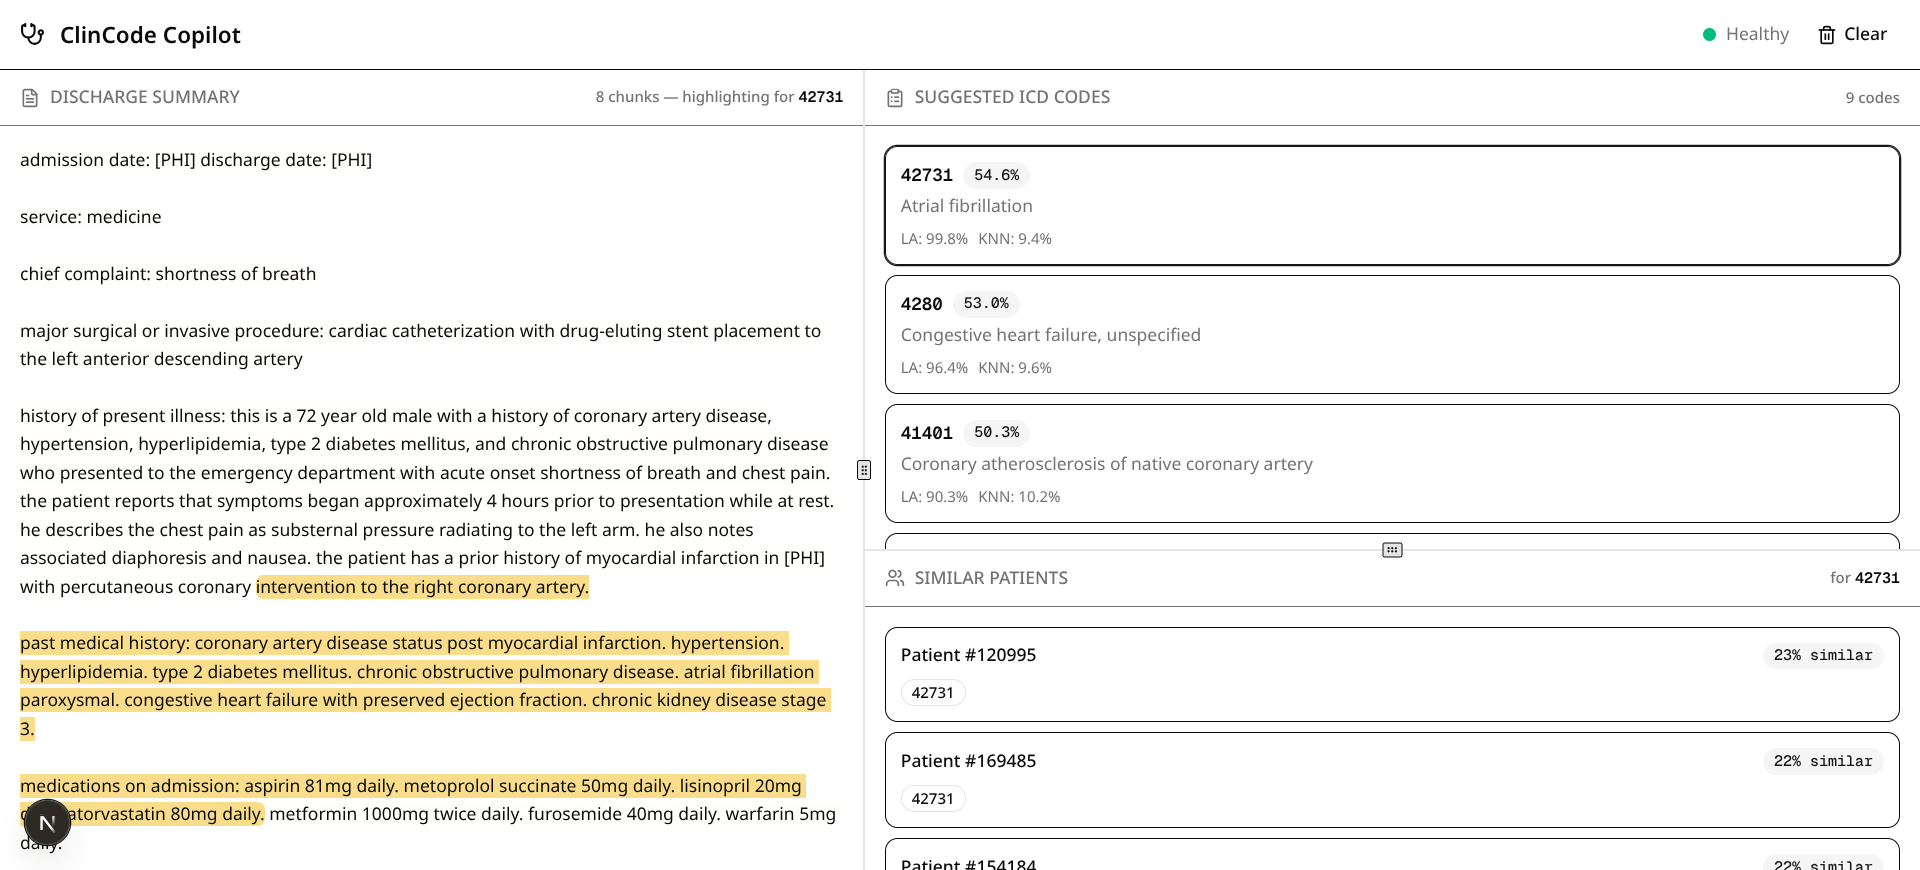
\includegraphics[width=0.95\textwidth]{figs/ui_overview.png}}
\caption{ClinCode Copilot workspace after analyzing a discharge summary. Left panel: clinical text with amber attention highlighting for ICD code 42731 (Atrial fibrillation), showing which document sections support the prediction. Top-right panel: predicted ICD codes ranked by ensemble confidence score, with individual label attention (LA) and KNN component scores. Bottom-right panel: similar training patients for the selected code, with similarity percentages.}
\label{fig:ui_overview}
\end{figure*}

\subsection{Backend}

The backend is implemented in Python using the FastAPI framework~\cite{b_fastapi}. At startup, a lifespan context manager loads all model artifacts into memory: the Bio\_ClinicalBERT encoder with its label attention head (approximately 110M parameters), the FAISS index containing 792,660 training chunk embeddings, associated metadata including sparse label matrices and admission identifiers, and a dictionary of 14,567 ICD-9 codes with descriptions.

The API exposes five endpoints. The \texttt{/api/predict} endpoint accepts a discharge text (minimum 50 characters) and returns predicted codes with ensemble scores, individual label attention and KNN scores, and ranks. The \texttt{/api/predict/detailed} endpoint extends this with per-code chunk attention weights, chunk text spans, and character-level span offsets that enable the frontend to map attention back to the original document. The \texttt{/api/similar-patients} endpoint accepts a text and a list of codes, returning the most similar training patients for each code along with similarity scores and shared code lists. The \texttt{/api/codes} endpoint supports paginated code search by code identifier or description, and \texttt{/api/codes/\{code\}} retrieves details for a specific code. All request and response schemas are defined using Pydantic models, providing runtime validation and automatic API documentation.

\subsection{ML pipeline}

The prediction pipeline operates in four stages. First, the input text is preprocessed: de-identification artifacts matching the pattern \texttt{[\textasteriskcentered\textasteriskcentered...\textasteriskcentered\textasteriskcentered]} are replaced with a placeholder token, horizontal whitespace is normalized, and the text is converted to lowercase. Second, the preprocessed text is segmented into overlapping chunks of 128 tokens (126 content tokens plus two special tokens) with a stride of 96 tokens (32-token overlap), retaining up to 20 chunks per document. The chunker records character-level span offsets for each chunk, enabling attention weights to be mapped back to positions in the original text.

Third, all chunks are encoded in a single batched forward pass through Bio\_ClinicalBERT~\cite{b_clinicalbert}. The encoder output is mean-pooled over the sequence dimension, projected from 768 to 256 dimensions, and L2-normalized. The label attention head computes per-code attention over the resulting chunk embeddings using 1,275 learned query vectors, producing both classification logits and attention weight distributions. Simultaneously, the chunk embeddings are searched against the FAISS index~\cite{b_faiss} to retrieve the 10 nearest training chunks by inner product similarity. Retrieved chunk labels are inherited from their parent documents, with each neighbor's similarity contribution divided by its parent document's total code count to prevent multi-coded documents from inflating scores. The per-code KNN score for the document is the maximum across its chunks.

Fourth, the ensemble combines scores through weighted averaging: $s_{\text{ens}} = 0.5 \cdot s_{\text{LA}} + 0.5 \cdot s_{\text{KNN}}$, and predictions exceeding a threshold of 0.4 are returned. The label attention and KNN components capture complementary signals: label attention aggregates evidence across all chunks through learned per-code queries, while KNN exploits local neighborhood structure at the individual chunk level.

\subsection{Frontend}

The frontend is implemented as a Next.js 16 application using React 19 and TypeScript. The workspace follows a multi-panel resizable layout implemented with the \texttt{react-resizable-panels} library. The horizontal split divides the viewport into a left panel (45\% default width, 25\% minimum) containing the discharge text, and a right panel (55\% default, 30\% minimum) that is further split vertically into a prediction list (60\% default height) and a similar patients panel (40\% default).

Client state---the current discharge text, prediction results, and selected code---is managed with Zustand~\cite{b_zustand}, while server state (API responses) is handled by TanStack React Query with a 30-second stale time. The UI is built with Radix UI primitives styled through Tailwind CSS, using the Geist typeface family. When a user enters discharge text and submits it, the frontend calls the detailed prediction endpoint. Upon receiving results, the first predicted code is automatically selected, and the left panel transitions from a text input to an attention-highlighted document viewer.

\section{Interpretability Features}

\subsection{Chunk-level attention visualization}

The primary interpretability mechanism maps the label attention model's per-code attention weights back to the original document as a visual heat-map overlay. When a user selects a predicted code from the prediction panel, the system retrieves that code's attention weight distribution over the document's chunks. Each chunk's attention weight is mapped to the character span it covers in the original text using the offsets computed during chunking. Where chunks overlap (due to the 32-token overlap stride), the maximum attention weight is assigned to each character position.

The resulting character-level weight array is segmented into contiguous spans of uniform weight, and each span is rendered with a background color whose intensity reflects the attention magnitude. The color scheme uses an amber hue (HSL 45\textdegree, 90\% saturation) with lightness and alpha modulated by the normalized weight: higher attention produces darker, more opaque highlighting. This section-level granularity---where each highlighted region corresponds to a contiguous 128-token chunk of the clinical note---is more actionable for clinical review than scattered token-level highlights, as it identifies coherent document sections (e.g., ``admission history,'' ``hospital course'') rather than individual words. Fig.~\ref{fig:ui_attention} illustrates how selecting a different code (41401, Coronary atherosclerosis) shifts the attention highlighting to different document sections compared to Fig.~\ref{fig:ui_overview}.

\begin{figure}[t]
\centerline{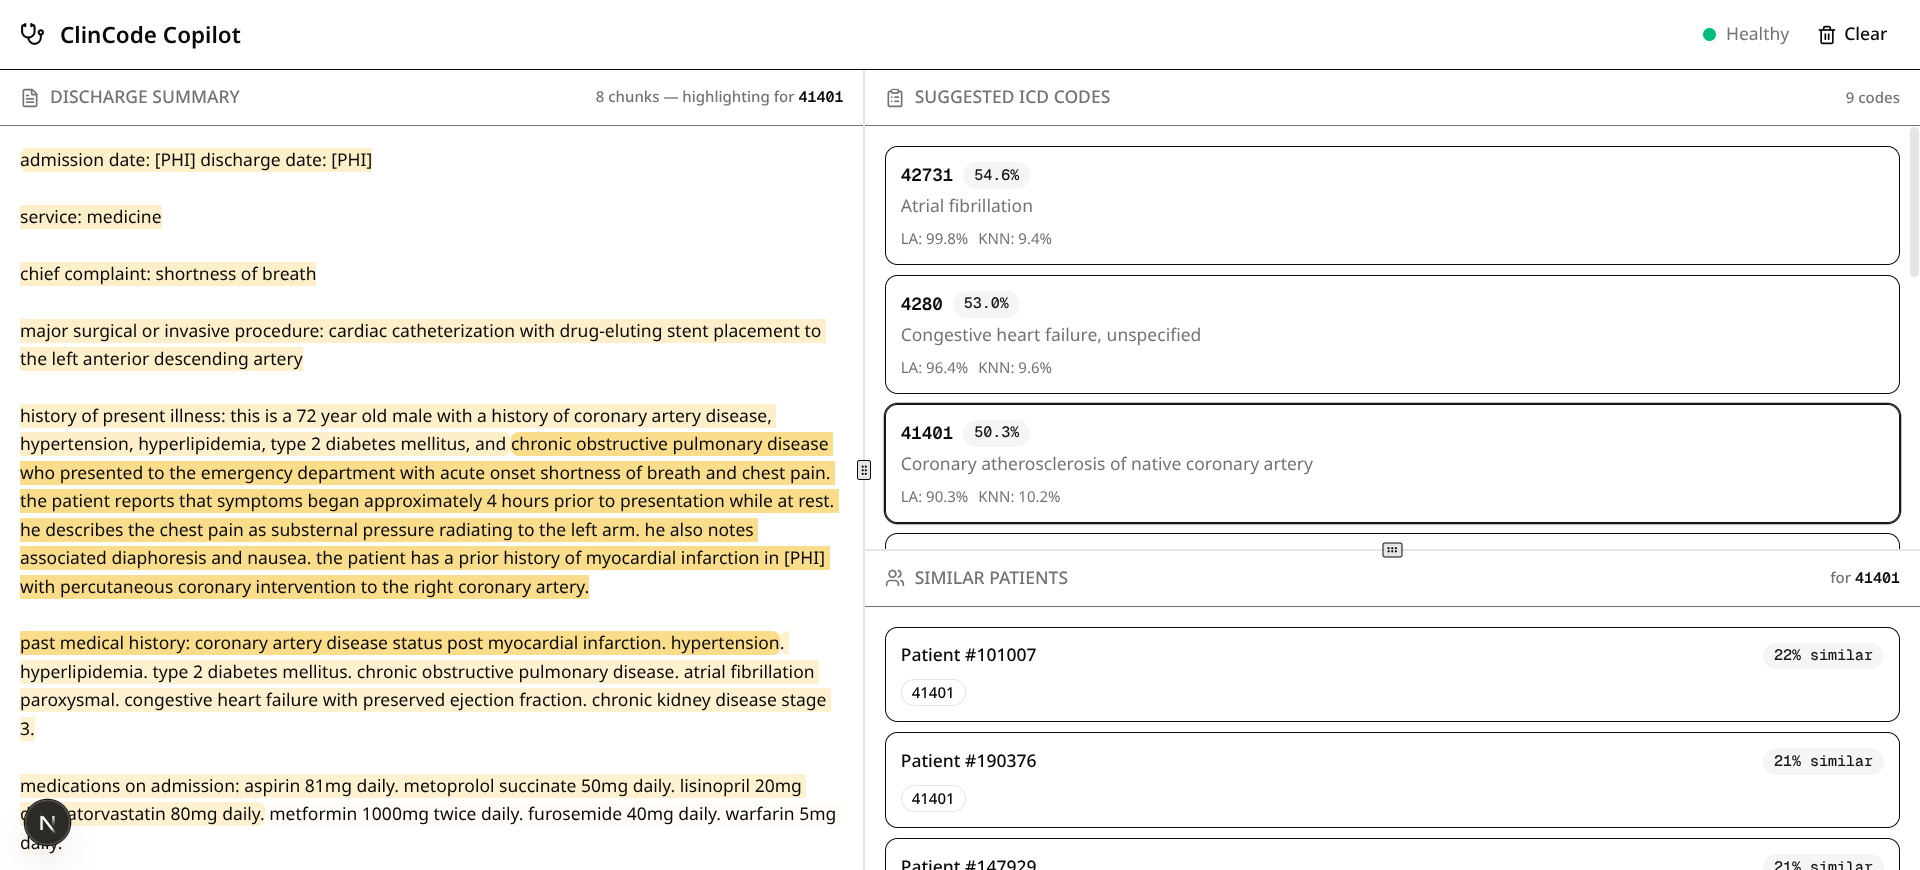
\includegraphics[width=\columnwidth]{figs/ui_attention_cad.png}}
\caption{Attention visualization for ICD code 41401 (Coronary atherosclerosis). Compared to code 42731 in Fig.~\ref{fig:ui_overview}, the attention distribution shifts to different document sections, demonstrating that each code attends to clinically relevant evidence.}
\label{fig:ui_attention}
\end{figure}

\subsection{Similar patient retrieval}

The second interpretability mechanism provides case-based reasoning through similar patient retrieval. When a code is selected, the frontend queries the \texttt{/api/similar-patients} endpoint, which encodes the input document's chunks and searches the FAISS index for training patients whose chunk embeddings are most similar. For each requested code, the system returns the training patients who received that code and whose chunks are nearest to the query document's chunks.

Each similar patient is displayed with its admission identifier, a similarity score (presented as a percentage), and a list of shared ICD codes rendered as badges. This information enables the clinical coder to perform case-based verification: if the most similar patients who received a particular code also share other codes with the current case, this increases confidence in the prediction. Conversely, if similar patients have a substantially different code profile, the coder may investigate further before accepting the prediction.

\subsection{Dual-mode workflow}

The two interpretability modes complement each other in clinical practice. Attention highlighting answers the question ``where in this document is the evidence for this code?'' by directing the coder's attention to specific sections. Similar patient retrieval answers the question ``what other patients received this code, and how similar are they?'' by providing empirical precedent. A clinical coder reviewing a prediction can first inspect the highlighted text sections to assess whether they contain appropriate clinical evidence, then examine similar patients to confirm that cases with comparable clinical profiles received the same code. This dual verification mirrors how experienced coders work: reading the note for evidence and recalling similar cases from experience.

The two modes also compensate for each other's limitations. Attention weights are indicative rather than causal~\cite{b_jain2019}, so high attention on a section does not guarantee that the model's prediction is correct for the reasons the coder assumes. Similar patient retrieval provides an independent signal: if the nearest training cases with the same code are highly similar, the prediction is likely correct regardless of whether the attention highlights the ``right'' sections.

\section{Implementation Details}

\subsection{Text preprocessing}

Clinical text from discharge summaries contains de-identification artifacts, inconsistent formatting, and protected health information (PHI) placeholders. The preprocessing pipeline addresses these through three transformations applied in sequence. First, de-identification patterns matching the regular expression \texttt{[\textbackslash*\textbackslash*...\textbackslash*\textbackslash*]} are replaced with a standardized \texttt{[PHI]} token. This handles the bracket-asterisk patterns used in de-identified clinical datasets such as MIMIC-III~\cite{b_mimic}. Second, horizontal whitespace (spaces, tabs) is normalized to single spaces while preserving line breaks that often delimit clinical sections. Third, sequences of three or more consecutive newlines are collapsed to double newlines. These transformations preserve the document's section structure while removing formatting artifacts that could interfere with tokenization.

\subsection{Deployment considerations}

Model loading occurs at application startup through FastAPI's lifespan context manager. The Bio\_ClinicalBERT encoder with label attention head occupies approximately 417 MB, and the FAISS IVF-Flat index with 792,660 vectors of 256 dimensions requires approximately 781 MB, plus 81 MB for associated metadata (sparse label matrices, admission identifiers). Total memory footprint at startup is approximately 1.3 GB. The FAISS index uses 100 inverted lists with 32 probes at query time, balancing search accuracy against latency for the approximate nearest-neighbor search.

The system is configured for CPU inference by default, with GPU support available through the \texttt{CLINCODE\_DEVICE} environment variable. On CPU, the computational bottleneck is the BERT forward pass over up to 20 chunks per document. Each chunk is 128 tokens, and the batched encoding processes all chunks in a single forward pass. The first 8 of 12 BERT layers are frozen (parameters fixed), which does not affect inference speed but reduces the model's trainable parameter count. The FAISS search over the IVF-Flat index with 32 probes is substantially faster than the encoding step, typically completing in single-digit milliseconds even on CPU.

\subsection{Technology stack}

The backend uses Python with FastAPI for the web framework, PyTorch for neural network inference, the Hugging Face Transformers library for the Bio\_ClinicalBERT tokenizer and model architecture, and FAISS (CPU version) for approximate nearest-neighbor search. Request and response schemas are defined with Pydantic v2, providing runtime validation, serialization, and automatic OpenAPI documentation. The ICD code dictionary---containing 14,567 ICD-9 codes with descriptions---is loaded as an in-memory JSON structure for constant-time lookups and substring search.

The frontend uses Next.js 16 with the App Router, React 19, and TypeScript. The resizable panel layout is implemented with \texttt{react-resizable-panels}. Component styling uses Tailwind CSS with Radix UI primitives following the shadcn/ui component pattern, which provides accessible, unstyled components that are customized through utility classes. State management is split between Zustand for client state (selected code, input text) and TanStack React Query for server state (API responses, with automatic caching and refetch management). The frontend communicates with the backend through a typed API client.

\section{Use Case and Evaluation}

\subsection{Clinical coding workflow}

ClinCode Copilot is designed to support the clinical coding workflow as an assistive tool rather than an autonomous system. The intended workflow proceeds as follows. A clinical coder pastes or enters a discharge summary into the left panel. Upon submission, the system returns predicted ICD codes ranked by confidence score in the prediction panel. The coder reviews each prediction in order: selecting a code highlights the supporting text sections in the discharge summary through the attention overlay, and the similar patients panel populates with training cases that received the same code. The coder can inspect the highlighted evidence, compare against similar cases, and make an informed decision to accept, reject, or modify each predicted code. An interactive code search dialog enables the coder to search the full ICD-9 vocabulary by code or description when manually adding codes not suggested by the model.

This workflow positions the system as a productivity tool that accelerates code identification while preserving the coder's decision-making authority. The dual interpretability features serve as evidence channels: attention highlights reduce the time needed to locate relevant clinical documentation, while similar patient retrieval provides empirical confidence calibration.

\subsection{Underlying model performance}

The hybrid model underlying ClinCode Copilot was trained on MIMIC-III~\cite{b_mimic} discharge summaries from 52,722 hospital admissions, split by patient into training (80\%), validation (10\%), and test (10\%) sets. Table~\ref{tab:performance} presents test set Micro-F1 at different minimum code frequency thresholds. The ensemble of label attention and chunk-level KNN achieves Micro-F1 of 0.482 on the full 1,275-code label space (minimum frequency 50), rising to 0.538 on the 374 codes covering 80\% of diagnoses and 0.563 on the 238 most frequent codes. The ensemble consistently outperforms both individual classifiers, with label attention contributing the majority of the signal and KNN providing complementary retrieval-based improvements of 0.7 to 2.1 Micro-F1 points across thresholds.

\begin{table}[t]
\caption{Micro-F1 on the MIMIC-III test set at different minimum code frequency thresholds. Coverage indicates the percentage of diagnosis assignments accounted for by codes at each threshold.}
\label{tab:performance}
\begin{center}
\begin{tabular}{r r c c c c}
\toprule
\textbf{Min-} & \textbf{\#} & \textbf{KNN} & \textbf{Label} & \textbf{Ensemble} & \textbf{Cov.} \\
\textbf{Freq} & \textbf{Codes} & & \textbf{Attn} & & \\
\midrule
50 & 1275 & 0.324 & 0.475 & \textbf{0.482} & 100\% \\
150 & $\sim$650 & 0.343 & 0.498 & \textbf{0.510} & $\sim$90\% \\
300 & 374 & 0.358 & 0.522 & \textbf{0.538} & 80.1\% \\
500 & 238 & 0.375 & 0.542 & \textbf{0.563} & 70.9\% \\
\bottomrule
\end{tabular}
\end{center}
\end{table}

These results reflect the same model deployed in the ClinCode Copilot system. The FAISS index contains the training chunk embeddings produced by the end-to-end encoder, and the label attention weights used for visualization are the same weights used for classification. No separate model is trained for explanation purposes---the interpretability features are a direct consequence of the model architecture.

\subsection{System performance}

Inference latency is dominated by the BERT encoding step, which processes up to 20 chunks of 128 tokens each in a single batched forward pass. On CPU (Intel Xeon-class processors), end-to-end prediction latency for a typical discharge summary ranges from 2 to 8 seconds depending on document length and chunk count. The FAISS IVF-Flat search with 32 probes across 792,660 vectors adds negligible latency (under 10 milliseconds). The detailed prediction endpoint, which additionally returns attention weights and chunk span mappings, incurs minimal overhead beyond the base prediction since the attention weights are already computed as part of the forward pass. The similar patients endpoint requires a separate FAISS search with post-processing to filter by requested codes and compute shared code lists. Total memory consumption at runtime is approximately 1.3 GB, enabling deployment on standard server hardware without GPU acceleration.

\section{Discussion}

ClinCode Copilot demonstrates that existing ICD coding models can be deployed as interactive tools with meaningful interpretability features when the model architecture is designed with explanation in mind. The chunk-level attention mechanism, originally chosen for classification efficiency, proves equally valuable as a user-facing explanation: attending over 20 chunk positions rather than thousands of tokens naturally produces section-level explanations that align with how clinical coders review documents.

The dual interpretability design addresses a fundamental challenge in clinical AI: no single explanation modality is sufficient. Attention weights provide spatial evidence (``where in the document'') but are indicative rather than causal~\cite{b_jain2019, b_wiegreffe2019}. Similar patient retrieval provides empirical evidence (``what similar cases received this code'') but does not explain what textual features drove the similarity. Together, they offer complementary perspectives that support informed clinical decision-making.

Several limitations should be acknowledged. The system cannot be demonstrated with real clinical data due to privacy restrictions on datasets such as MIMIC-III, limiting evaluation to offline metrics rather than user studies with clinical coders. The attention-as-explanation paradigm has known caveats: high attention on a text section does not guarantee that the model's prediction depends causally on that section~\cite{b_jain2019}, though alternative explanations (e.g., gradient-based attribution) would require additional computation that may compromise real-time interaction. The fixed ensemble threshold of 0.4 represents a single operating point; in practice, different clinical settings may require different precision-recall tradeoffs, and the system does not currently expose threshold configuration to end users.

The section-level granularity of chunk attention (128 tokens per chunk) may be too coarse when the relevant evidence is a single phrase or lab value within a chunk. A hybrid approach that combines chunk-level attention for initial section identification with token-level attribution within the attended chunks could provide finer-grained explanations without the computational cost of full document token-level attention. Additionally, the similar patient retrieval currently shows admission identifiers without clinical context beyond shared codes; enriching the display with summary information about similar cases would improve the case-based reasoning workflow.

Future work includes conducting user studies with clinical coders to evaluate the utility of dual explanations in practice, integrating the system with electronic health record (EHR) platforms for seamless workflow integration, exploring active learning from coder feedback to improve model performance over time, and extending the system to support ICD-10 coding vocabularies.

\section{Conclusion}

We presented ClinCode Copilot, an interactive clinical coding assistant that combines a hybrid ICD coding model with a web-based workspace designed for real-time code review and verification. The system provides dual interpretability through chunk-level attention visualization and similar patient retrieval, enabling clinical coders to inspect supporting evidence for each predicted code. Built with a FastAPI backend serving Bio\_ClinicalBERT and FAISS, and a Next.js frontend with a resizable multi-panel layout, the system achieves Micro-F1 of 0.482 on 1,275 MIMIC-III ICD-9 codes while maintaining real-time inference on CPU hardware. ClinCode Copilot demonstrates that bridging the gap between automated coding models and clinical workflow requires not only accurate predictions but also interactive explanations that support the coder's decision-making process.

\FloatBarrier
\bibliographystyle{IEEEtran}
\bibliography{references}

\end{document}
